\documentclass{article}

\usepackage[letterpaper]{geometry}
\usepackage{graphicx}

\graphicspath{{./img/}}

\title{2411 HW 11}
\author{Duncan Wilkie}
\date{23 November 2021}

\begin{document}

\maketitle

\section{}
The program appears in the script files section. Plots of the value of each of the RNGs against their previous value appear below.
\[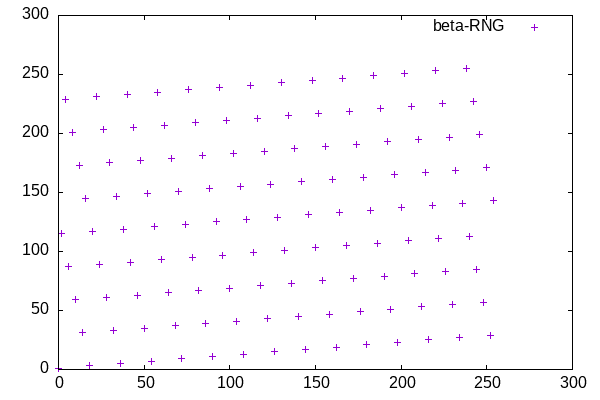
\includegraphics[scale=.6]{beta.png}\]
\[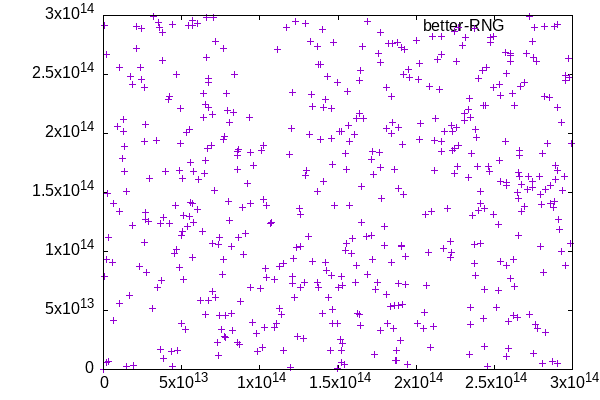
\includegraphics[scale=.6]{better.png}\]
It is evident the second RNG is less correlated than the first.

\section{}
The seed is the first value, which is 1. The period is the number of elements it takes before the sequence repeats itself, in this case 8. The next number in the sequence is therefore 4. To generate uniform random numbers in $[-1,1]$, we take the values of the RNG, divide by the period to get a floating-point RNG over $[0,1]$, and then apply the transformation $x\mapsto 2x-1$ to get a floating-point RNG over $[-1,1]$. Doing this, the first two numbers of the RNG become $-0.75$ and $0.5$.

\end{document}
%%% Local Variables:
%%% mode: latex
%%% TeX-master: t
%%% End:
